\section{Segmentation}
We now explain how execution is split into segments.

\subsection{Execution Segments}

\begin{figure}
\centering
\resizebox{0.99\textwidth}{!}{%
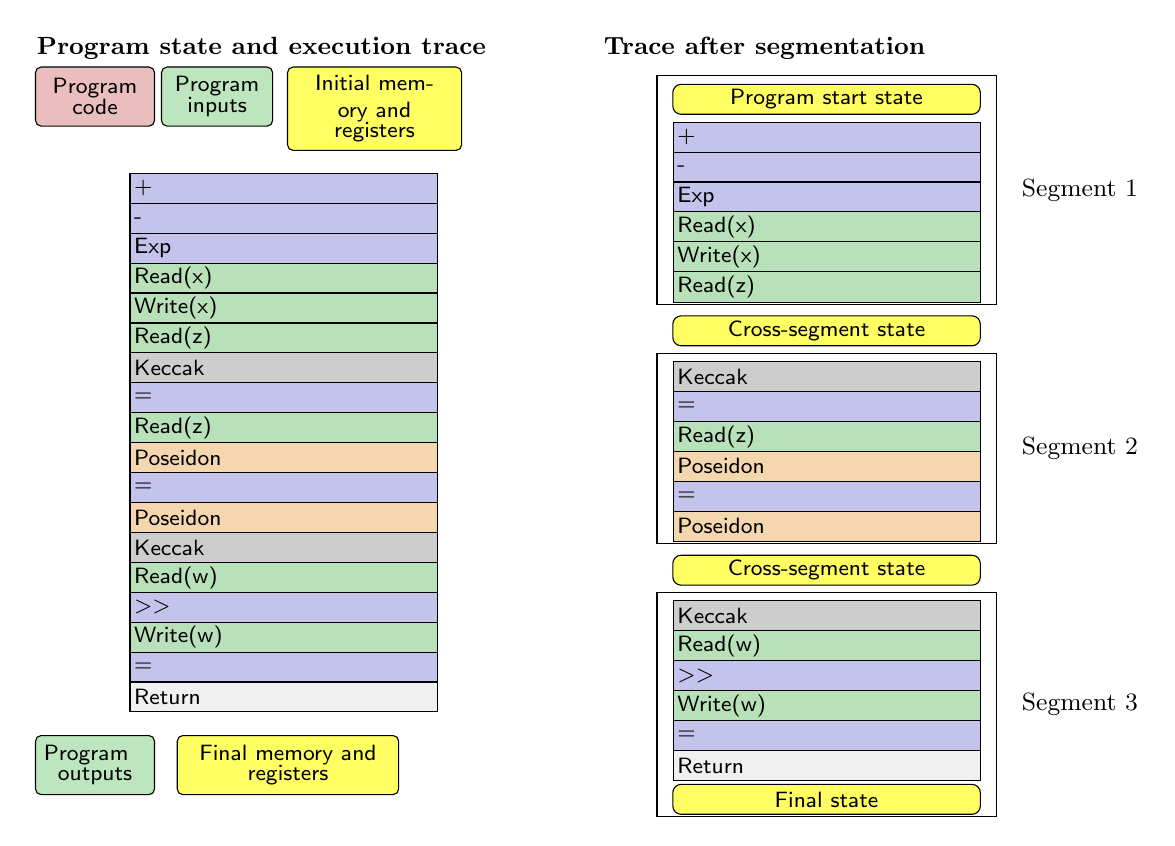
\begin{tikzpicture}[y=-1cm]
  % Colors
  \definecolor{alucol}{RGB}{195,195,235}
  \definecolor{memcol}{RGB}{185,225,185}
  \definecolor{hashcol}{RGB}{205,205,205}
  \definecolor{poscol}{RGB}{245,215,175}
  \definecolor{retcol}{RGB}{240,240,240}
  \definecolor{codecol}{RGB}{235,190,190}
  \definecolor{inputcol}{RGB}{190,230,190}
  \definecolor{statecol}{RGB}{255,255,100}
  %
  \def\rh{0.38}
  \def\bw{3.8cm}
  %
  \tikzset{
    ibox/.style={draw, thin, minimum height=\rh cm, text width=\bw, inner sep=1.5pt,
                 anchor=north west, font=\footnotesize\sffamily},
    sbox/.style={draw, thin, rounded corners=3pt, fill=statecol, minimum height=0.38cm,
                 text width=\bw, align=center, inner sep=1.5pt, font=\footnotesize\sffamily,
                 anchor=north},
    tbox/.style={draw, thin, rounded corners=2pt, minimum height=0.75cm, inner sep=3pt,
                 font=\footnotesize\sffamily, align=center, anchor=north west},
    seglabel/.style={font=\small, anchor=west},
  }
  %
  %%% LEFT SIDE %%%
  \node[anchor=north west, font=\small\bfseries] at (0, 0) {Program state and execution trace};
  %
  % Top boxes
  \node[tbox, fill=codecol, text width=1.3cm] at (0.1, 0.5) {Program\\[-2pt]code};
  \node[tbox, fill=inputcol, text width=1.2cm] at (1.7, 0.5) {Program\\[-2pt]inputs};
  \node[tbox, fill=statecol, text width=2.0cm] at (3.3, 0.5) {Initial memory and\\[-2pt]registers};
  %
  % Left instruction list (18 rows)
  \def\ly{1.85}
  \def\lx{1.3}
  \foreach \n/\txt/\col in {
    0/{+}/alucol, 1/{-}/alucol, 2/{Exp}/alucol,
    3/{Read(x)}/memcol, 4/{Write(x)}/memcol, 5/{Read(z)}/memcol,
    6/{Keccak}/hashcol, 7/{=}/alucol, 8/{Read(z)}/memcol,
    9/{Poseidon}/poscol, 10/{=}/alucol, 11/{Poseidon}/poscol,
    12/{Keccak}/hashcol, 13/{Read(w)}/memcol,
    14/{\textgreater\textgreater}/alucol, 15/{Write(w)}/memcol,
    16/{=}/alucol, 17/{Return}/retcol%
  } {
    \node[ibox, fill=\col] at (\lx, {\ly+\n*\rh}) {\txt};
  }
  %
  % Bottom boxes
  \node[tbox, fill=inputcol, text width=1.3cm] at (0.1, {\ly+18*\rh+0.3}) {\raggedright Program\\[-2pt]outputs};
  \node[tbox, fill=statecol, text width=2.6cm] at (1.9, {\ly+18*\rh+0.3}) {Final memory and\\[-2pt]registers};
  %
  %%% RIGHT SIDE %%%
  \def\rx{8.2}
  \pgfmathsetmacro{\rcx}{\rx + 1.953}
  %
  \node[anchor=north west, font=\small\bfseries] at (7.2, 0) {Trace after segmentation};
  %
  % --- Segment 1 ---
  \def\startY{0.72}
  \node[sbox] at (\rcx, \startY) {Program start state};
  %
  \pgfmathsetmacro{\segAy}{\startY + 0.48}
  \foreach \n/\txt/\col in {
    0/{+}/alucol, 1/{-}/alucol, 2/{Exp}/alucol,
    3/{Read(x)}/memcol, 4/{Write(x)}/memcol, 5/{Read(z)}/memcol%
  } {
    \node[ibox, fill=\col] at (\rx, {\segAy+\n*\rh}) {\txt};
  }
  %
  \pgfmathsetmacro{\segAtop}{\startY - 0.1}
  \pgfmathsetmacro{\segAbot}{\segAy + 6*\rh + 0.04}
  \draw[thin] ({\rx-0.2}, \segAtop) rectangle ({\rx+3.8+0.11+0.2}, \segAbot);
  \node[seglabel] at ({\rx+3.8+0.11+0.4}, {(\segAtop+\segAbot)/2}) {Segment 1};
  %
  % --- Cross-segment state 1 ---
  \pgfmathsetmacro{\isAy}{\segAbot + 0.14}
  \node[sbox] at (\rcx, \isAy) {Cross-segment state};
  %
  % --- Segment 2 ---
  \pgfmathsetmacro{\segBy}{\isAy + 0.58}
  \foreach \n/\txt/\col in {
    0/{Keccak}/hashcol, 1/{=}/alucol, 2/{Read(z)}/memcol,
    3/{Poseidon}/poscol, 4/{=}/alucol, 5/{Poseidon}/poscol%
  } {
    \node[ibox, fill=\col] at (\rx, {\segBy+\n*\rh}) {\txt};
  }
  %
  \pgfmathsetmacro{\segBtop}{\segBy - 0.1}
  \pgfmathsetmacro{\segBbot}{\segBy + 6*\rh + 0.04}
  \draw[thin] ({\rx-0.2}, \segBtop) rectangle ({\rx+3.8+0.11+0.2}, \segBbot);
  \node[seglabel] at ({\rx+3.8+0.11+0.4}, {(\segBtop+\segBbot)/2}) {Segment 2};
  %
  % --- Cross-segment state 2 ---
  \pgfmathsetmacro{\isBy}{\segBbot + 0.14}
  \node[sbox] at (\rcx, \isBy) {Cross-segment state};
  %
  % --- Segment 3 ---
  \pgfmathsetmacro{\segCy}{\isBy + 0.58}
  \foreach \n/\txt/\col in {
    0/{Keccak}/hashcol, 1/{Read(w)}/memcol,
    2/{\textgreater\textgreater}/alucol, 3/{Write(w)}/memcol,
    4/{=}/alucol, 5/{Return}/retcol%
  } {
    \node[ibox, fill=\col] at (\rx, {\segCy+\n*\rh}) {\txt};
  }
  %
  \pgfmathsetmacro{\finalY}{\segCy + 6*\rh + 0.05}
  \node[sbox] at (\rcx, \finalY) {Final state};
  %
  \pgfmathsetmacro{\segCtop}{\segCy - 0.1}
  \pgfmathsetmacro{\segCbot}{\finalY + 0.42}
  \draw[thin] ({\rx-0.2}, \segCtop) rectangle ({\rx+3.8+0.11+0.2}, \segCbot);
  \node[seglabel] at ({\rx+3.8+0.11+0.4}, {(\segCtop+\segCbot)/2}) {Segment 3};
\end{tikzpicture}%
}
\caption{Segmentation of the execution trace into 3 segments }\label{img:trace-seg}
\end{figure}

After execution, the execution trace $\TTT$ is divided into segments $\GGG_1,\GGG_2,\ldots,\GGG_m$
of exactly $N_{\text{seg}}$ instructions\footnote{The instruction
set has a no-op instruction to pad the segment to the full length.
The parameter $N_{\text{seg}}$ is assumed to be hardcoded and fixed, and known to the verifier.} each (cf. Fig. \ref{img:trace-seg}). Each segment $\GGG_i$ corresponds to a contiguous
subsequence of the execution trace, from $S_{start_i}$ to $S_{end_i}$, and is proven by a set of separate
proofs.
The segmentation of the execution trace into consecutive segments
allows reducing the proof of the entire execution to proving the validity of each segment
and consistency between them. The global consistency argument asserts that the segments are consistent with each other
and with the public inputs/outputs:
$$
S_{end_i} = S_{start_{i+1}}\text{ for all }i\in[m-1],\quad S_{start_1}=S_0,\quad S_{end_m}=S_T.
$$

\subsection{Segment layout}

Each segment is represented in an equivalent form as a collection of one trace and several
\emph{chips}, listed below (cf.\ Fig.~\ref{img:segments}).


\paragraph{Segment trace}
It consists of all  operations of the execution trace within
the segment and state variables, including the program counter, register values, memory state, etc.
It is a collection of $N_{\text{seg}}$ rows, each corresponding to one instruction step
from the segment. The segment trace does not enforce the semantics of all instructions,
but only a subset of them, and the rest of the instructions are proven
in separate chips  and their consistency with the segment trace is enforced by
\emph{consistency arguments}.

\paragraph{Keccak chip}  It consists of all Keccak precompile calls in the segment, and their inputs/outputs.

\paragraph{Poseidon chip}
It consists of all Poseidon precompile calls in the segment, and their inputs/outputs.

\paragraph{Range check chip}
It consists of all range check statements occurring in the segment.

\paragraph{Local consistency argument}$\phantom{=}$

\begin{instruction}
  Teams should describe how their bus consistency argument works in terms of lookups used and how they integrate into the overall proof system.
\end{instruction}

The consistency arguments enforce that the operations proven in the chips are consistent
with the segment trace. This is done using the concept of a \emph{bus} connecting the segment trace and the chips,
and lookup arguments to enforce consistency of the bus values with the segment trace and the chip traces.

\begin{figure}
\centering
\resizebox{0.65\textwidth}{!}{%
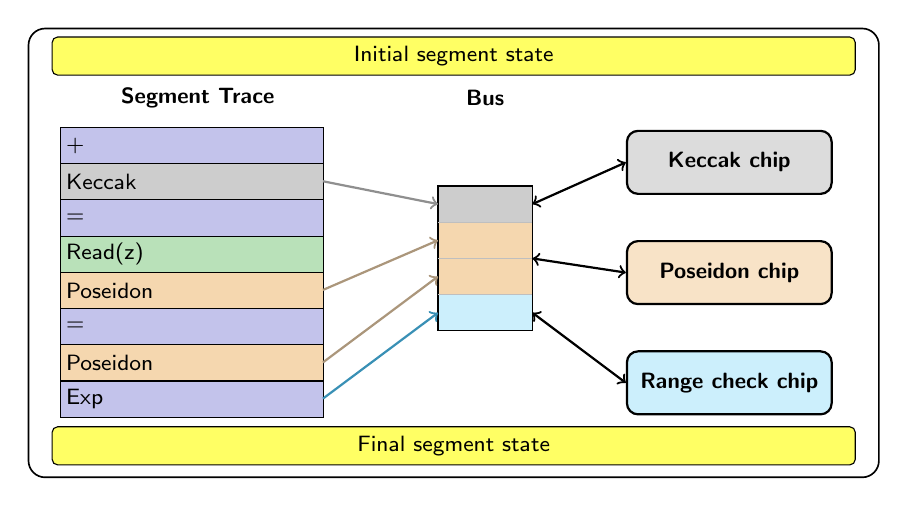
\begin{tikzpicture}[y=-1cm]
  % Colors
  \definecolor{alucol}{RGB}{195,195,235}
  \definecolor{memcol}{RGB}{185,225,185}
  \definecolor{hashcol}{RGB}{205,205,205}
  \definecolor{poscol}{RGB}{245,215,175}
  \definecolor{statecol}{RGB}{255,255,100}
  \definecolor{buscol}{RGB}{255,195,115}
  %
  \def\rh{0.46}
  %
  \tikzset{
    ibox/.style={draw, thin, minimum height=\rh cm, text width=3.2cm, inner sep=2pt,
                 anchor=north west, font=\footnotesize\sffamily},
    chip/.style={draw, thick, rounded corners=4pt, minimum width=2.6cm, minimum height=0.8cm,
                 font=\footnotesize\sffamily\bfseries, align=center},
    sbar/.style={draw, thin, rounded corners=2pt, fill=statecol,
                 minimum height=0.42cm, minimum width=10.2cm,
                 font=\footnotesize\sffamily},
  }
  %
  % Layout constants
  \def\tx{0.4}     % trace x
  \def\trw{3.34}   % trace box total width (3.2 text + 0.14 inner sep)
  \def\busx{5.2}   % bus x (shifted right for arrow space)
  \def\busw{1.2}   % bus width
  \def\ty{1.25}    % trace y start
  \def\bsy{2.0}    % bus start y (shorter than trace)
  %
  % === BIG ENCLOSING BOX ===
  \draw[semithick, rounded corners=6pt] (0, 0) rectangle (10.8, 5.7);
  %
  % === INITIAL STATE BAR ===
  \node[sbar] at (5.4, 0.35) {Initial segment state};
  %
  % === COLUMN LABELS ===
  \node[font=\footnotesize\sffamily\bfseries] at (2.15, 0.88) {Segment Trace};
  \node[font=\footnotesize\sffamily\bfseries] at ({\busx + \busw/2}, 0.88) {Bus};
  %
  % === INSTRUCTION ROWS (color-coded by chip affiliation) ===
  \foreach \n/\txt/\col in {
    0/{+}/alucol,
    1/{Keccak}/hashcol,
    2/{=}/alucol,
    3/{Read(z)}/memcol,
    4/{Poseidon}/poscol,
    5/{=}/alucol,
    6/{Poseidon}/poscol,
    7/{Exp}/alucol%
  } {
    \node[ibox, fill=\col] at (\tx, {\ty+\n*\rh}) {\txt};
  }
  %
  % === BUS COLUMN (only precompile/range-check entries, colored by chip) ===
  % 4 cells: Keccak, Poseidon, Poseidon, Range check
  \fill[hashcol]  (\busx, \bsy) rectangle ({\busx+\busw}, {\bsy+\rh});
  \fill[poscol]   (\busx, {\bsy+\rh}) rectangle ({\busx+\busw}, {\bsy+2*\rh});
  \fill[poscol]   (\busx, {\bsy+2*\rh}) rectangle ({\busx+\busw}, {\bsy+3*\rh});
  \fill[cyan!20]  (\busx, {\bsy+3*\rh}) rectangle ({\busx+\busw}, {\bsy+4*\rh});
  % Grid
  \draw[thin] (\busx, \bsy) rectangle ({\busx+\busw}, {\bsy+4*\rh});
  \foreach \n in {1,2,3} {
    \draw[thin, black!25] (\busx, {\bsy+\n*\rh}) -- ({\busx+\busw}, {\bsy+\n*\rh});
  }
  %
  % === ARROWS: TRACE → BUS ===
  \pgfmathsetmacro{\trR}{\tx + \trw}  % trace right edge
  % Keccak (trace row 1) → bus cell 0
  \draw[->, thick, hashcol!70!black] (\trR, {\ty+1*\rh+\rh/2}) -- (\busx, {\bsy+\rh/2});
  % Poseidon (trace row 4) → bus cell 1
  \draw[->, thick, poscol!70!black] (\trR, {\ty+4*\rh+\rh/2}) -- (\busx, {\bsy+\rh+\rh/2});
  % Poseidon (trace row 6) → bus cell 2
  \draw[->, thick, poscol!70!black] (\trR, {\ty+6*\rh+\rh/2}) -- (\busx, {\bsy+2*\rh+\rh/2});
  % Exp/range check (trace row 7) → bus cell 3
  \draw[->, thick, cyan!70!black] (\trR, {\ty+7*\rh+\rh/2}) -- (\busx, {\bsy+3*\rh+\rh/2});
  %
  % === FINAL STATE BAR ===
  \node[sbar] at (5.4, 5.3) {Final segment state};
  %
  % === CHIP BOXES (spread across full trace height) ===
  \node[chip, fill=hashcol!70] (sha3chip) at (8.9, 1.7) {Keccak chip};
  \node[chip, fill=poscol!70] (poschip) at (8.9, 3.1) {Poseidon chip};
  \node[chip, fill=cyan!20] (rangechip) at (8.9, 4.5) {Range check chip};
  %
  % === ARROWS: BUS → CHIPS (bidirectional) ===
  \draw[<->, thick] ({\busx+\busw}, {\bsy+\rh/2}) -- (sha3chip.west);
  \draw[<->, thick] ({\busx+\busw}, {\bsy+2*\rh}) -- (poschip.west);
  \draw[<->, thick] ({\busx+\busw}, {\bsy+3*\rh+\rh/2}) -- (rangechip.west);
  %
\end{tikzpicture}%
}
\caption{Segment structure: segment trace connects to the bus which then connects to chips.}\label{img:segments}
\end{figure}

